\documentclass[12pt]{article}
\usepackage[margin=1in]{geometry}
\usepackage{amsmath}
\usepackage{amsthm}
\usepackage{float}
\usepackage{graphicx}
\usepackage{multirow}
\usepackage{natbib}
\usepackage{tabularx} 
\usepackage{enumitem}
\usepackage{array}
\usepackage{booktabs}
\usepackage{hyperref}
\usepackage[utf8]{inputenc}
\usepackage{lipsum}
\usepackage[english]{babel}
\usepackage[autostyle, english = american]{csquotes}
\usepackage{underscore}
\MakeOuterQuote{"}
\title{Call Center Regression Data Analysis}

\author{Michael  Marcaccio}

\date{November 14 2022}

\begin{document}

\maketitle

\begin{abstract}
 With over 15 million people employed, a predicted compound annual growth rate (CAGR) of 5.6 percent between 2020 and 2027, and with over 28,000 locations
 in the United States alone, call centers play a pivotal role in a business' success.In this paper, call center volume was forecasted and
 models were created to predict the number of agents needed to meet critical attributes such as waittime, calltime, and holdtime. 
 Forecasting gives businesses the ability to make informed business decision and develop data-driven strategies. In the literature it is very
 common to see call center volume being predicted using different techniques, but there is very limited studies on attempting to correlate
 the number of agents needed. Through Regression techniques, there are 8 models proposed to model the number of agents needed based on waittime,
 calltime, goaltime, and the amount of calls handled.
\end{abstract}

\section*{Introduction}
  With over 15 million people employed, a predicted compound annual growth rate (CAGR) of 5.6 percent between 2020 and 2027, and with over 28,000 locations
in the United States alone, call centers play a pivotal role in a business' success. Call centers are a key part of customer service
that will save a company time, money, and unneccessary obstacles. In the banking industry, calls can range from inquires, transfers, 
payments, reporting, to processing. This means members could call about their account balance, credit card bills, loan applications, 
or unauthorized transactions. It is crucial that a bank is prepared for spikes in calls and have agents knowledgeable in all aspects of banking.


  Many studies have been done working with call center volumes as presented in Modeling and Forecasting Call Center Arrivals \citep{ibrahim2016modeling}.
Here an Autoregressive moving average (ARIMA) model is used, which is depicted in the paper as:
\begin{equation}
  \label{eq:ARIMA Standard}
  \Phi(B)(x_i -\mu)=\theta_q(B)\varepsilon_t
\end{equation}
Ibrahim uses multiple ARIMA models to depict seasonality with a combination of exponential smoothing. Holt-Winters smoothing is also used,
with three equations of:
\begin{equation}
  \label{eq:Holt-Winters}
  M_t=\alpha_0(X_t-S_{t-s}) + (1-\alpha_0)(M_{t-1}+B_{t-1}),
\end{equation}
\begin{equation}
  \label{eq:Holt-Winters2}
  B_t=\alpha_1(M_t-M_{t-1}) +(1-\alpha_1)B_{t-1},
\end{equation}
\begin{equation}
  \label{eq:Holt-Winters3}
  S_t=\alpha_2(X_t-M_t) +(1-\alpha_2)S_{t-s},
\end{equation}
where $B_{t}$ is the slope component, $M_{t}$ is the level component, $S_{t}$ is the seasonal component, and s is the period of seasonality.
ARIMA models are a great model to create as "they allow the  representation of a  wide array of potentially useful predictor functions in  models  which contain relatively few parameters" \citep{newbold1983arima}.
With the combination of Holt-Winters smoothing, Ibrahim creates a great model for forecasting call volume, however the paper never goes into detail about
how many agents there should be working at a set time. 

  \citep{evensen1999effective} goes into detail about effective service delivery stating the expectations of customers are a "function of
the customer's own experiences...and when judging their own service quality, financial instiutions need to evalute themselves on 
objective measures which span across industries".When taking this into consideration, I focused my models on using a calls per agent approach,
so agents are not overworked and can treat each caller with respect while answering their concerns in a timely manner to represent the business in a good light. \citep{avramidis2005modeling} confirms
this as it is described as the "call-to-agent assignment problem", and that an efficiency-driven call center is important.


  The contributions of the paper creates models on the basis to maximize quality of service in relation to the number of agents. 
Based on this, models were created to minimize:
\begin{enumerate}
  \item Wait Time
  \item Call Time
  \item Reduce the Amount of Agent Handle Time
  \item Reduce the Amount of Calls not being handled
\end{enumerate}
The remainder of the paper will present the dataset and break it into a clear view on the historical data. I have also created a 
forecast on the projected call volume throughout a week on 15 minute intervals.


\section*{Data}
\begin{sloppypar}
  The data comes from an undisclosed bank where I wrote two SQL queries to obtain. This comes directly from the banks records dating back from Febuary 2020
  to Septemeber 2022, and I was lucky enough to do a data analysis on real-life data. This dataset consists of 466,565 observations of 31 variables. 
  Some significant variables consist of Calldate, Caller_ID, Caller_ID, QueuedYN, AnsweredYN, AbandonedYN, QueuedName, InteractionOutcome, 
  AnsweredGoalMet, StartTime, EndTime, WaitTime, Holdtime, AgentTalkDuration, AgentHandleTime, WrapUpTime, DayoftheYear,
  WeekoftheYear, and NbrofAgents.
\end{sloppypar}
  It is important to acknowledge that AgentTalkDuration refers to the actual amount of time the agent the agent was talking while
AbandonedYN refers to if the caller ended the call before speaking to a representative. The QueuedYN is if the member was put in a queue and had to wait to speak to an agent.
The queue is an automated service or an IVR (Interactive Voice Response). The latest generation of speech-recognition technology allows
IVRs to interpret complex user commands, so customers may be able to “self-serve”, i.e., complete the service interaction at the IVR. \citep{avramidis2005modeling}.
Holdtime is how long the member waits when an agent places on them hold, while waittime is how long they have to wait before someone answers there call.
WrapUpTime refers to how long the member takes to hang up the phone after the agent stops talk. AgentHandleTime is the total of Holdtime, WrapUpTime, and AgentTalkDuration combined.

  This data is allows me to easily answer the research question as I am using real-life data. With a huge sample size and many variables,
there is a great opportunity for data analysis and modeling. With this dataset, I know when doing calculations such as finding means and creating plots, 
they will able to accurately give a truly image of call center volume and agent information to a small period of time such as 15 minutes.
  I did do some exploratory data analysis by creating figures that represent call center volume by the year, month, day of week, and time. 
I also created a tabled that shows the average wait time, talk time, hold time, wrap up time, and count of every interaction Outcome.
\begin{figure}[H]
  \centering
  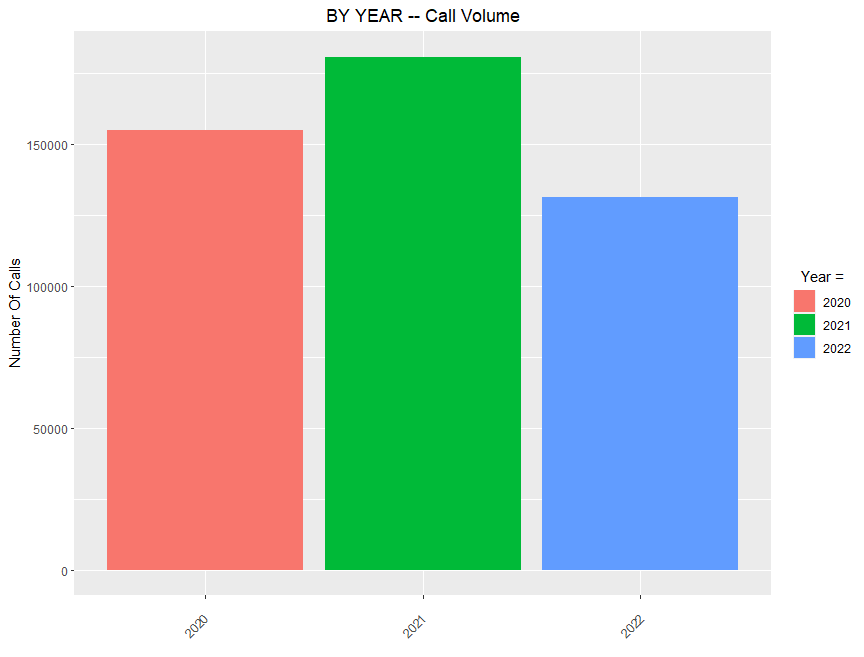
\includegraphics[width=\textwidth]{By Year.png}
  \caption{Call Volume Grouped by Year.}
  \label{fig:Year}
\end{figure}
Here we can see that 2021 has the highest call volume. Please Note that 2020 only has 11 months, while 2020 only has 10. This may be why the data appears skewed.
\begin{figure}[H]
  \centering
  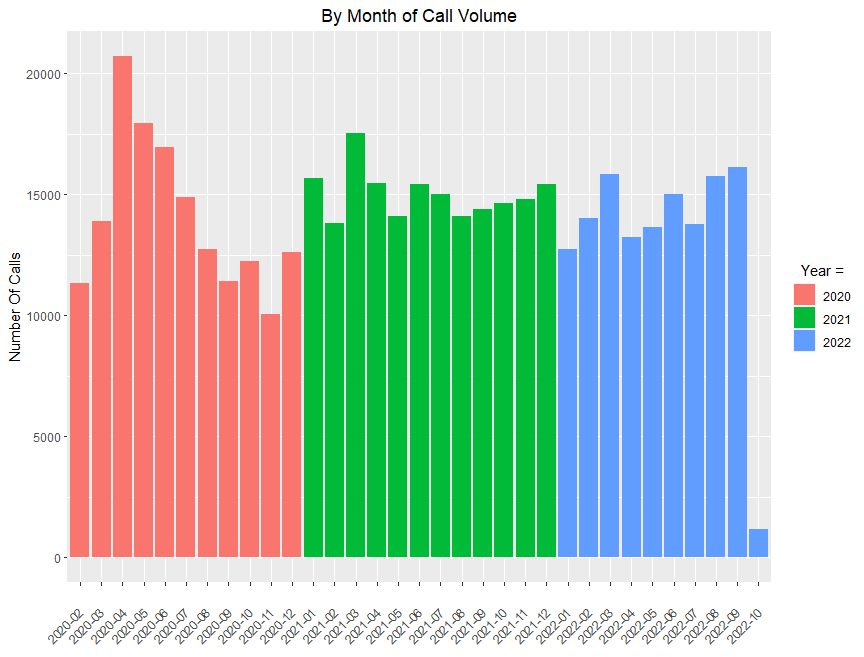
\includegraphics[width=\textwidth]{ByMonthVolume.png}
  \caption{Call Volume Grouped by Month.}
  \label{fig:Month}
\end{figure}
When grouped by month, we can see an interesting peak around April. This may be because that is tax season and members are calling for tax information.
Also April 2020 may have a higher peak than April 2021, due to COVID-19. During that time, many individuals were eligble for a 1,200 dollar stimulus check.
\begin{figure}[H]
  \centering
  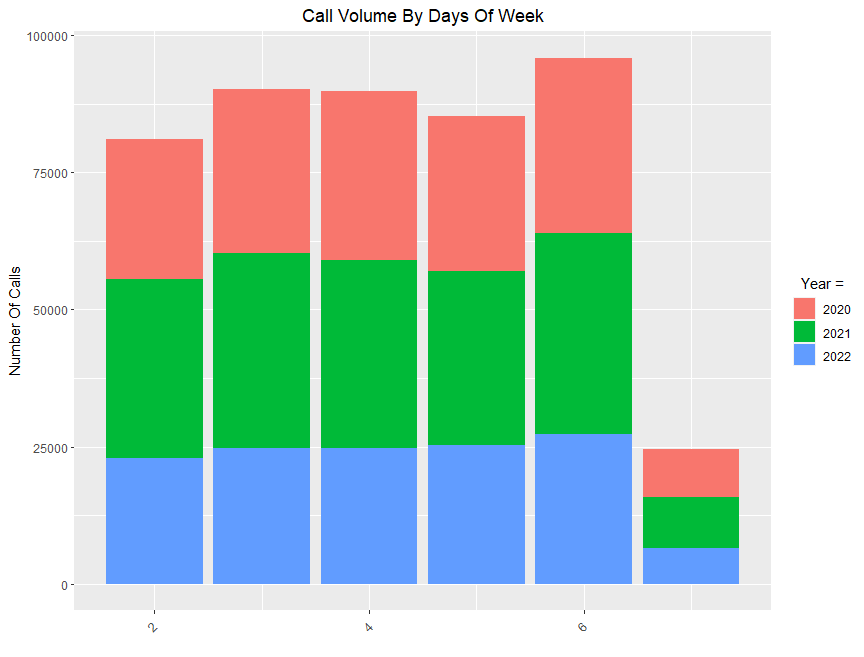
\includegraphics[width=\textwidth]{CallVolumeByDayOfWeek.png}
  \caption{Call Volume Grouped by Day.}
  \label{fig:Day}
\end{figure}
With Sunday representing 1, we can see that most calls happen on a Friday. Saturday has an extremely low count. This can be explained due to the
varying hours of the call center. Monday through Thursday, the call center is open 8am to 5pm, a total of 9 hours. Friday the call center is open
8am-7pm, a total of 11 hours. Saturday the call center is only open 8:30 am to 12pm, a total of 3 and a half hours.
\begin{figure}[H]
  \centering
  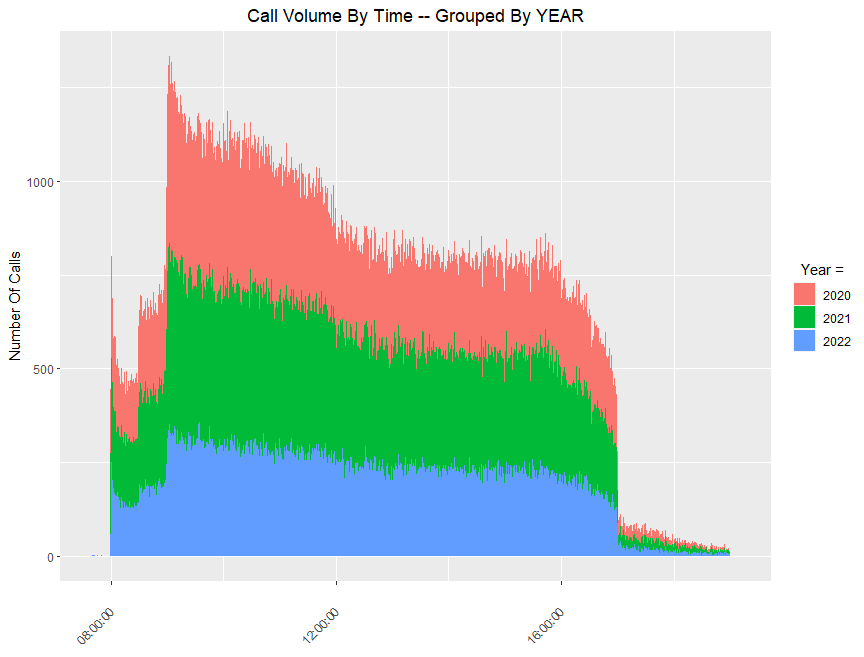
\includegraphics[width=\textwidth]{CallVolumeByTimeOfDayGROUPEDbyYear.png}
  \caption{Call Volume Grouped by Time.}
  \label{fig:Timeoneday}
\end{figure}
The call center consistently has a spike around 9am throughout the 3 years. This is suprising as the call center opens at 8am. This is important to be aware of when
creating a forecasting model and having the banks employees be at their station at 9am. The decreasing trend throughout the day is not suprising
as most people are working throughout the day.
\begin{table}[H]
  \resizebox{\textwidth}{!} {
  \begin{tabular}{ l | l | l | l | l | l | l}
    {\bf Outcome} & {\bf Count} & {\bf Wait Avg} & {\bf Talk Avg} & {\bf Hold Avg} & {\bf Wrap Avg} & {\bf Total Talk Avg} \\
  \hline
  Abandoned & 2364 & 100 & 11.3 & 0.06 & 2.40 & 13.8 \\
  \hline
  Handled & 460047 & 107 & 253 & 26.2 & 16.3 & 295\\
  \hline
  Leave Number & 411 & 214 & 66 & 6.18 & 7.80 & 80\\
  \hline
  Not Specified & 299 & 1.21 & 120 & 0.278 & 3.24 & 123\\
  \hline
  Service Unavailable & 1 & 0 & 0 & 0 & 0 & 0\\
  \hline
  Wrong Number & 3 & 357 & 0 & 0 & 12 & 12\\
  \end{tabular}
  }
  \end{table}
Here it is prevalent that a majority of calls are handled. These variables played a key part in my models for the agents.
\section*{Methods}
I created linear models to show the relationship between calls per agent and average waitime, holdtime, average goal met, and average 
interaction value. Average goal met was a variable created in relationship to the AnsweredGoalMet. AnsweredGoalMet was given in 1 and 0s, 
1 if the goal was hit and 0 if it was not hit. This variable is very fluid, as each company has its own reasoning for what they want their
goal time to be. Average Interaction Value was based off a variable that was created based on the InteractionOutcome. "Handled "got assigned 
1 as it was a positive outcome and -1 for "Abandoned" and "Leave Number" as they were deemed negative. The others were considered neutral, for example
"Not Specified", was given a 0. 
Linear Regression is based off five key assumptions, there is a linear relationship, multivariate normality, No or little multicollinearity, No auto-correlation, 
and Homoscedasticity. multicollinearity refers to 

\section*{Simulation}



\section*{Discussion}


\bibliographystyle{chicago}
\bibliography{Citations.bib}
\end{document}